\documentclass{beamer}
 
\usepackage[utf8]{inputenc}
\usepackage{braket}
\usepackage{mathtools} % Needed for \prescript
\usetheme{boxes}
\setbeamertemplate{navigation symbols}{}
\usepackage{subfig}
\usepackage{hyperref}
\usepackage{xcolor}

\captionsetup[subfigure]{labelformat=empty}
\captionsetup[figure]{labelformat=empty}

\newcommand{\tot}{\mathrm{tot}}
\DeclareMathOperator{\Tr}{Tr}

%Information to be included in the title page:
\title{STIR and Tensorflow}
\author{Philipp Windischhofer}
%\institute{ETH Zürich}
\date{July 27, 2017}
  
\begin{document}
 
\frame{\titlepage}

\section{The big picture}
\begin{frame}
  \frametitle{The big picture}
  \begin{itemize}
    \item STIR
    \item iterative reconstruction algorithms
    \item find the optimum of a \textsl{cost function}\\
      \begin{align*} P(\text{global LOR response} | \text{image}) = \prod_{\text{all LORs}} P(\text{LOR response} | \text{image})\end{align*}\\
      \begin{align*} P(\text{LOR response} | \text{image}) = \int_{\text{LOR}} \text{image density}\end{align*}
      \item Image (estimate) $\leadsto$ LOR response: \textsl{forward projection}
  \end{itemize}
\end{frame}

\begin{frame}
  \frametitle{Ray tracing}
  \begin{itemize}
    \item in the following: how to compute / \underline{approximate} this integral?
    \item represent \textsl{image} as a discretized array of voxels
    \begin{align*}\int_{\text{LOR}} \text{image density} \leadsto \sum_{\text{traversed voxels}} \text{LOI} \cdot \text{voxel brightness}\end{align*}
    \item $\text{LOI} = $ \underline{length of intersection} of the LOR through a specific voxel
  \end{itemize}
  (Standard) STIR spends $>$ 90\% of the reconstruction time for \textsl{forward projection}
  \begin{itemize}
    \item is there a way to make it faster?
  \end{itemize}
\end{frame}

\begin{frame}
\frametitle{Table of Contents}
\tableofcontents
\end{frame}

\section{Tensorflow - what is it?}
\begin{frame}
\frametitle{Tensorflow}
\begin{itemize}
  \item \textsl{Google}: ``An open-source software library for machine intelligence''
    \begin{itemize}
      \item heavily used in the machine-learning community
    \end{itemize}
  \item Much more than that:
    \begin{itemize}
      \item a software package for numerical calculations using data-flow \textsl{graphs}
    \end{itemize}

    \begin{figure}
      \centering
      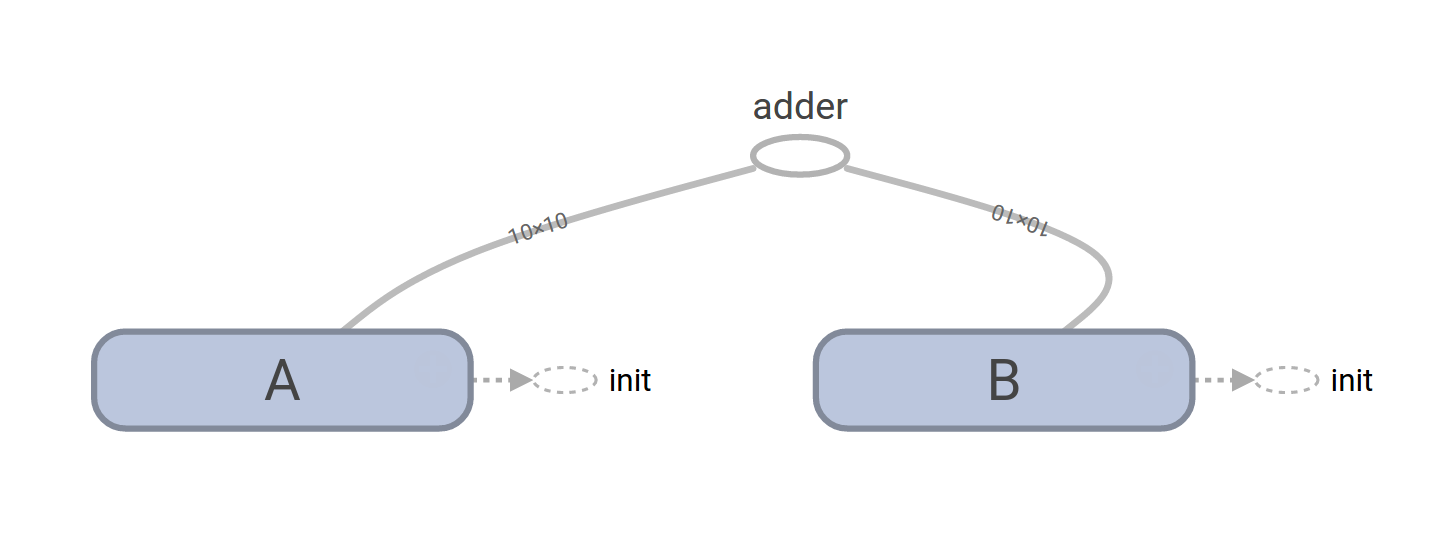
\includegraphics[width = 0.9\textwidth]{../ExampleGraph.png}
    \end{figure}

    \begin{itemize}
      \item Design the graph \textsl{now}, save it to a file, run it \textsl{later}...
      \item Can run it (almost) everywhere: CPU, GPU, a cluster, ...
    \end{itemize}
\end{itemize}
\end{frame}

\section{How to do ray tracing on a CPU?}
\begin{frame}
  \frametitle{How to do ray tracing on a CPU?}
  \framesubtitle{Siddon's algorithm (2D)}
  \begin{figure}
    \centering
    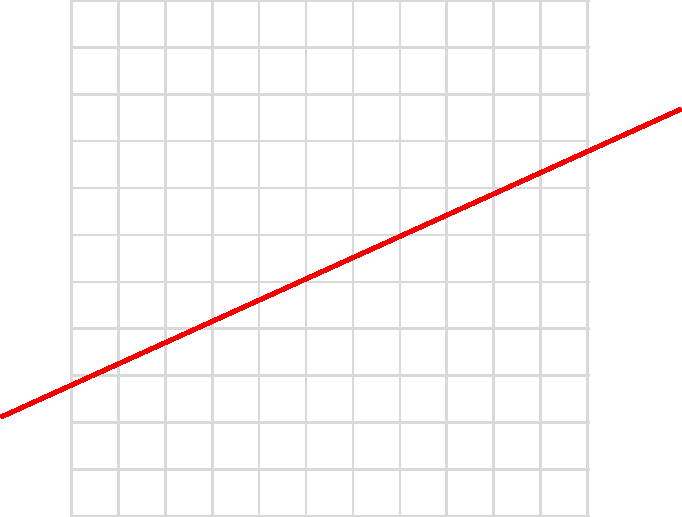
\includegraphics[width = 0.7\textwidth]{../Siddon.pdf}
  \end{figure}
  \begin{itemize}
    \item a (very) sequential algorithm
  \end{itemize}
\end{frame}

\begin{frame}
  \frametitle{How to do ray tracing on a CPU?}
  \framesubtitle{Siddon's algorithm (2D)}
  \begin{figure}
    \centering
    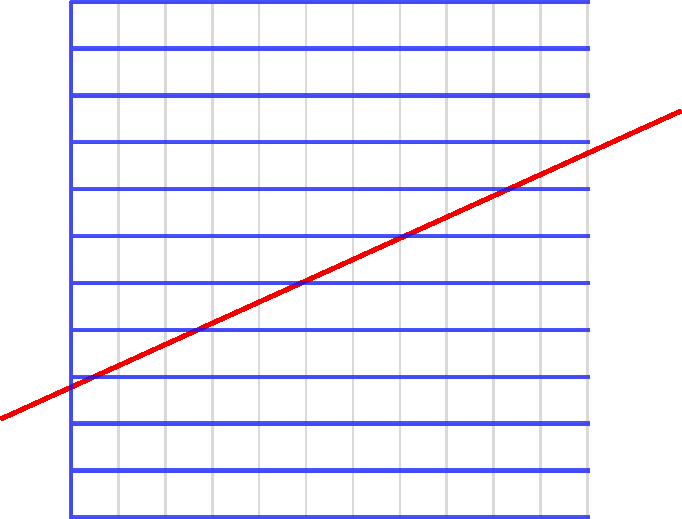
\includegraphics[width = 0.7\textwidth]{../Horizontal.pdf}
  \end{figure}
  \begin{itemize}
    \item get intersections of LOI with all horizontal planes
  \end{itemize}
\end{frame}

\begin{frame}
  \frametitle{How to do ray tracing on a CPU?}
  \framesubtitle{Siddon's algorithm (2D)}
  \begin{figure}
    \centering
    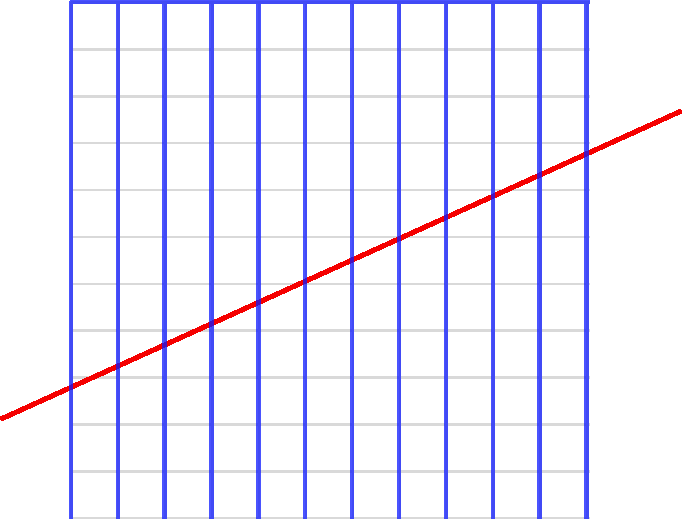
\includegraphics[width = 0.7\textwidth]{../Vertical.pdf}
  \end{figure}
  \begin{itemize}
    \item get intersections of LOI with all vertical planes
  \end{itemize}
\end{frame}

\begin{frame}
  \frametitle{How to do ray tracing on a CPU?}
  \framesubtitle{Siddon's algorithm (2D)}
  \begin{figure}
    \centering
    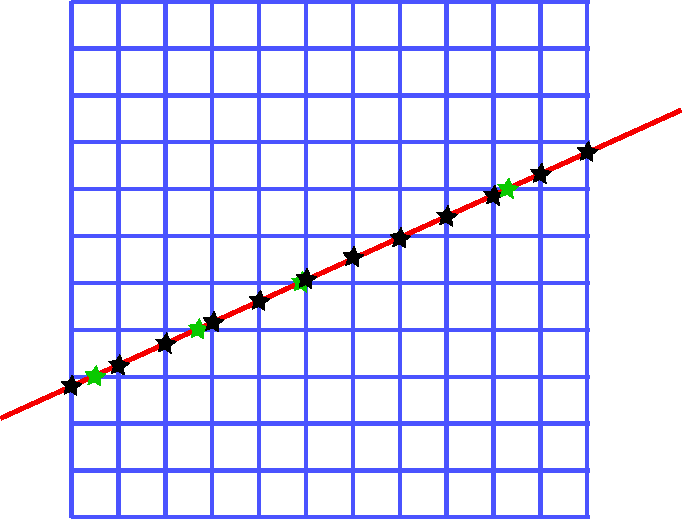
\includegraphics[width = 0.7\textwidth]{../SiddonTraced.pdf}
  \end{figure}
  \begin{itemize}
    \item combine them and get the individual LOIs
  \end{itemize}
\end{frame}

\begin{frame}
  \frametitle{How to do ray tracing on a CPU?}
  \framesubtitle{Siddon's algorithm (2D)}
  \begin{itemize}
    \item parametrize the LOR
      \begin{align*} \mathbf{x} = (\mathbf{x_{end}} - \mathbf{x_{start}}) \cdot \alpha + \mathbf{x_{start}} \end{align*}
      \begin{align*} \alpha \in [0,1] \end{align*}
    \item get intersections with horizontal and vertical planes in terms of the line parameter $\alpha$
    \item merge and sort them
    \item \textsl{differences} between neighbouring $\alpha$ values in the merged list describe the LOIs!
  \end{itemize}
\end{frame}

\section{How to do ray tracing on a GPU?}
\begin{frame}
  \frametitle{Siddon and Tensorflow}
  \begin{itemize}
    \item Siddon: $\mathcal{O}(N)$ for a LOR of length $N$ (this means a voxel array of size $N^3$!!)
    \item many branches, a loop over the LOR, ...
    \item \underline{very} inefficient when running with Tensorflow (GPU $\neq$ CPU architecture)
      \begin{itemize}
        \item especially problematic when trying to trace multiple LORs ``in parallel''
      \end{itemize}

    \item for Tensorflow: need an algorithm that ...
      \begin{itemize}
        \item uses the same algorithmic steps on \textsl{all} voxels of the LOR
        \item uses the same algorithmic steps on \textsl{all} LORs
      \end{itemize}
  \end{itemize}
\end{frame}

\begin{frame}
  \frametitle{Alternatives to Siddon}
  \begin{itemize}
    \item naive approach: for every LOR, compute the LOI through \textsl{every} voxel, then add them all up
      \begin{itemize}
        \item works fine with Tensorflow, but scales as $\mathcal{O}(N^3)$
        \item CPU \& Siddon beat it again for real-world array sizes
      \end{itemize}
    \item alternative approach: think of (intersection) points \textsl{without} the notion of an LOR
  \end{itemize}
  \begin{figure}
    \centering
    \only<1>{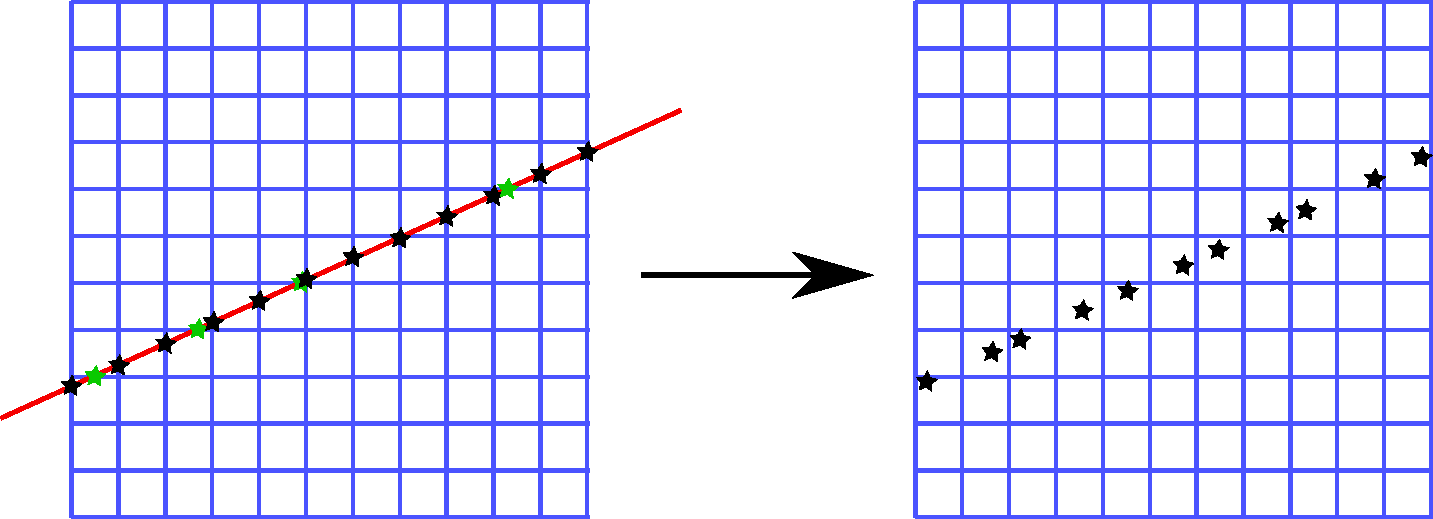
\includegraphics[width = 0.9\textwidth]{../RMPointsLOR.pdf}}
    \only<2>{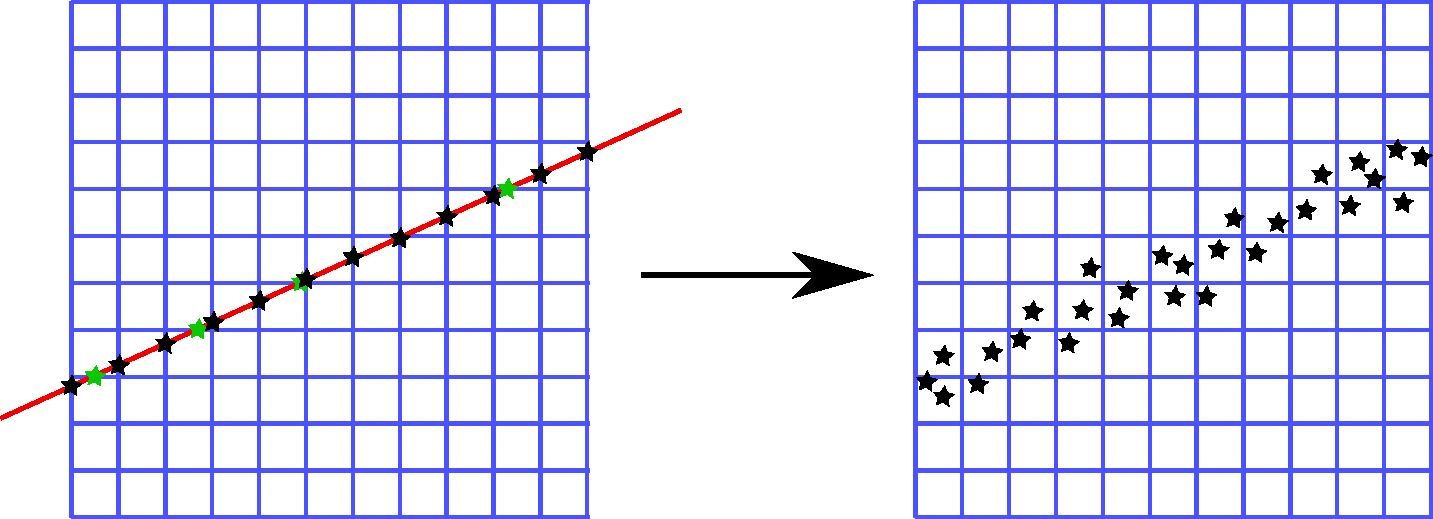
\includegraphics[width = 0.9\textwidth]{../RMPointsTOR.pdf}}
  \end{figure}
\end{frame}

\begin{frame}
  \frametitle{Voxel-by-voxel LOI calculation}
  \begin{itemize}
    \item still not much easier than the full problem!
    \item a cube is very discontinuous, hard to do it analytically without branches
    \item what if content with an \textsl{approximate} solution?
  \end{itemize}

  \begin{figure}
    \centering
    \only<1>{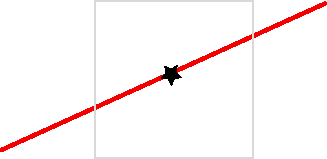
\includegraphics[width = 0.9\textwidth]{../RayMarchingStep0.pdf}}
    \only<2>{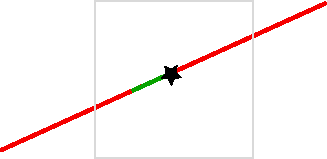
\includegraphics[width = 0.9\textwidth]{../RayMarchingStep1.pdf}}
    \only<3>{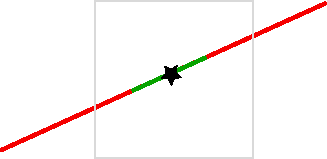
\includegraphics[width = 0.9\textwidth]{../RayMarchingStep2.pdf}}
    \only<4>{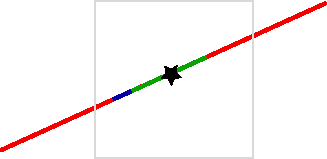
\includegraphics[width = 0.9\textwidth]{../RayMarchingStep3.pdf}}
    \only<5>{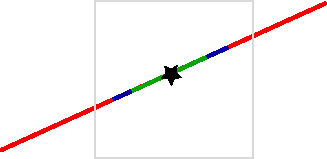
\includegraphics[width = 0.9\textwidth]{../RayMarchingStep4.pdf}}
  \end{figure}
\end{frame}

\begin{frame}
  \frametitle{Ray marching: an iterative algorithm}
  \begin{itemize}
    \item Use \textsl{signed distance function} of a cube to cut down the number of iterations that are needed
      \begin{itemize}
        \item a heuristic that produces an \textsl{underestimation} of the distance to the voxel boundary
      \end{itemize}
      \item need to assess the residual error that remains
  \end{itemize}
\end{frame}

\begin{frame}
  \frametitle{Ray marching: an iterative algorithm}
  \framesubtitle{Accuracy}
  \begin{itemize}
    \item assume: have ``enough'' points along the LOR
  \end{itemize}
  \begin{figure}
    \centering
    \subfloat[][]{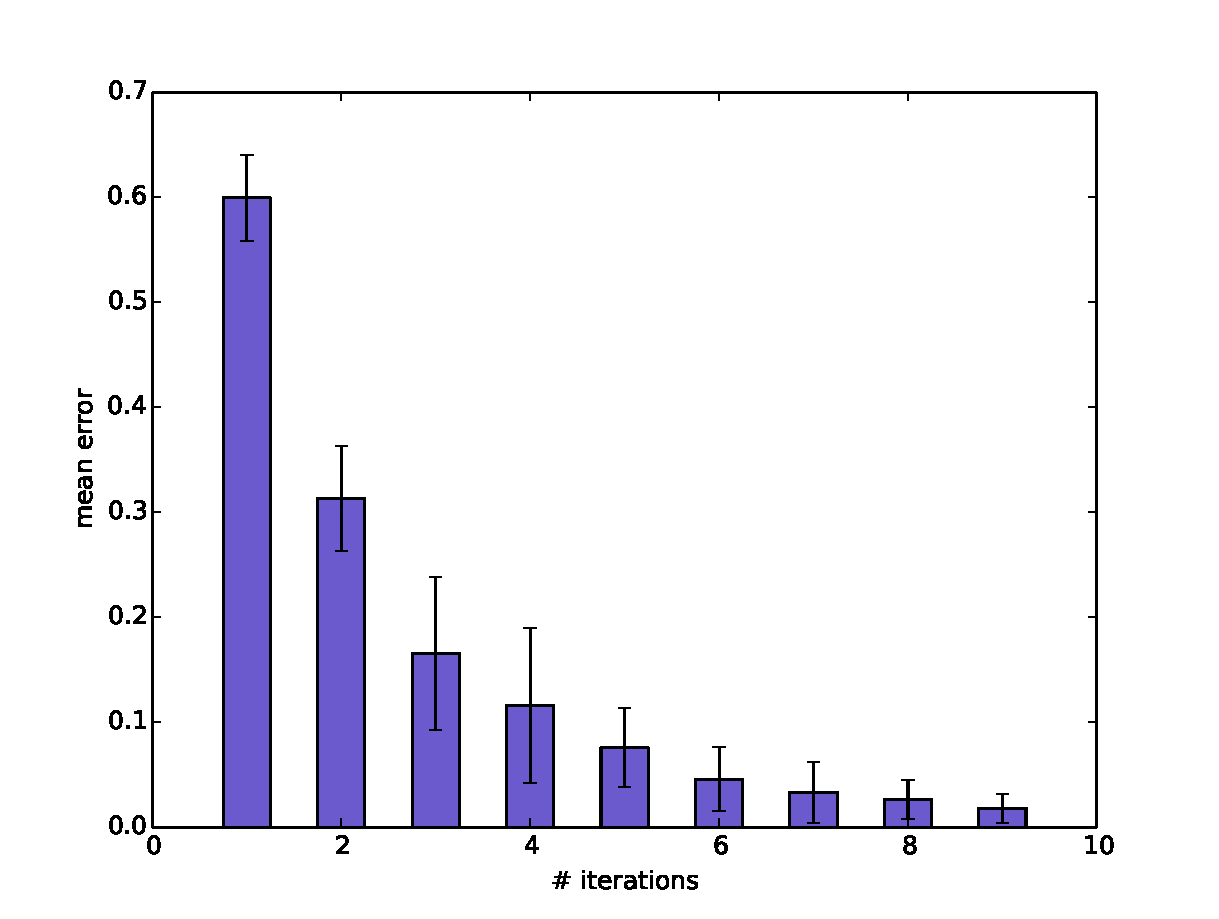
\includegraphics[width = 0.7\textwidth]{../iterations.pdf}\label{6its}}
  \end{figure}
  \begin{itemize}
    \item with 6 iterations, are already at $\sim$ 5\% level!
  \end{itemize}
\end{frame}

\begin{frame}
  \frametitle{Ray marching: an iterative algorithm}
  \framesubtitle{Accuracy}
  \begin{itemize}
    \item are there ever enough points?
  \end{itemize}
  % put 3d histogram here

  \begin{itemize}
    \item does not matter for STIR!
  \end{itemize}
\end{frame}

\begin{frame}
  \frametitle{Bringing together STIR and Tensorflow}
  \framesubtitle{The infrastructure}
  \begin{itemize}
    \item Build the Tensorflow graph in a Python script
      \begin{itemize}
        \item much easier and faster to prototype
        \item Python API much better documented and more stable
      \end{itemize}
    \item \underline{Save} the complete graph into a \texttt{ProtoBuf} file
    \item \underline{Load} the file using the C++ API and make use of it in STIR
      \begin{itemize}
        \item link STIR against the Tensorflow (shared) library
      \end{itemize}
  \end{itemize}
\end{frame}

\section{Results}
\begin{frame}
  \frametitle{Speedup without caching}
  \begin{figure}
    \centering
      \subfloat[][]{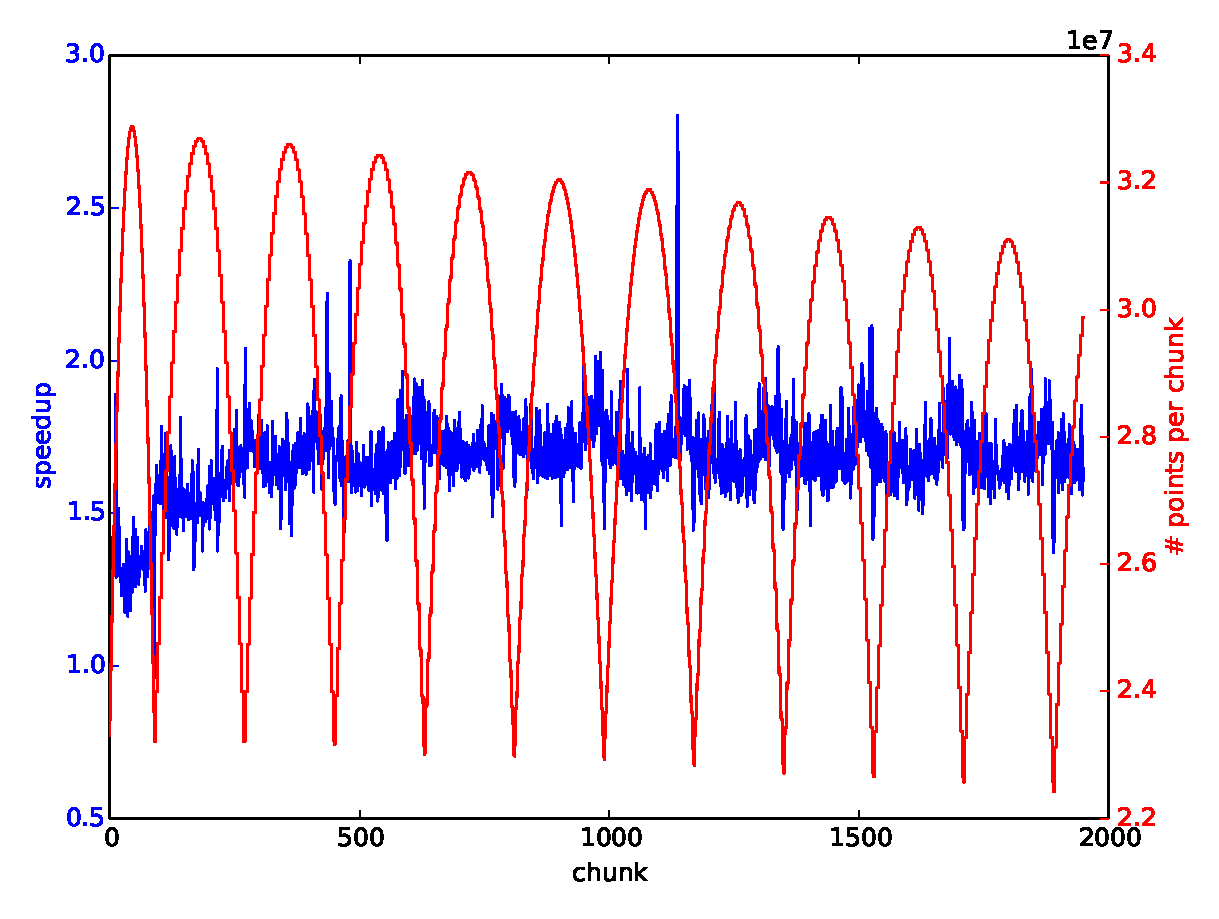
\includegraphics[width = 0.52\textwidth]{../speedup_6_iterations.pdf}\label{6its}}
      \subfloat[][]{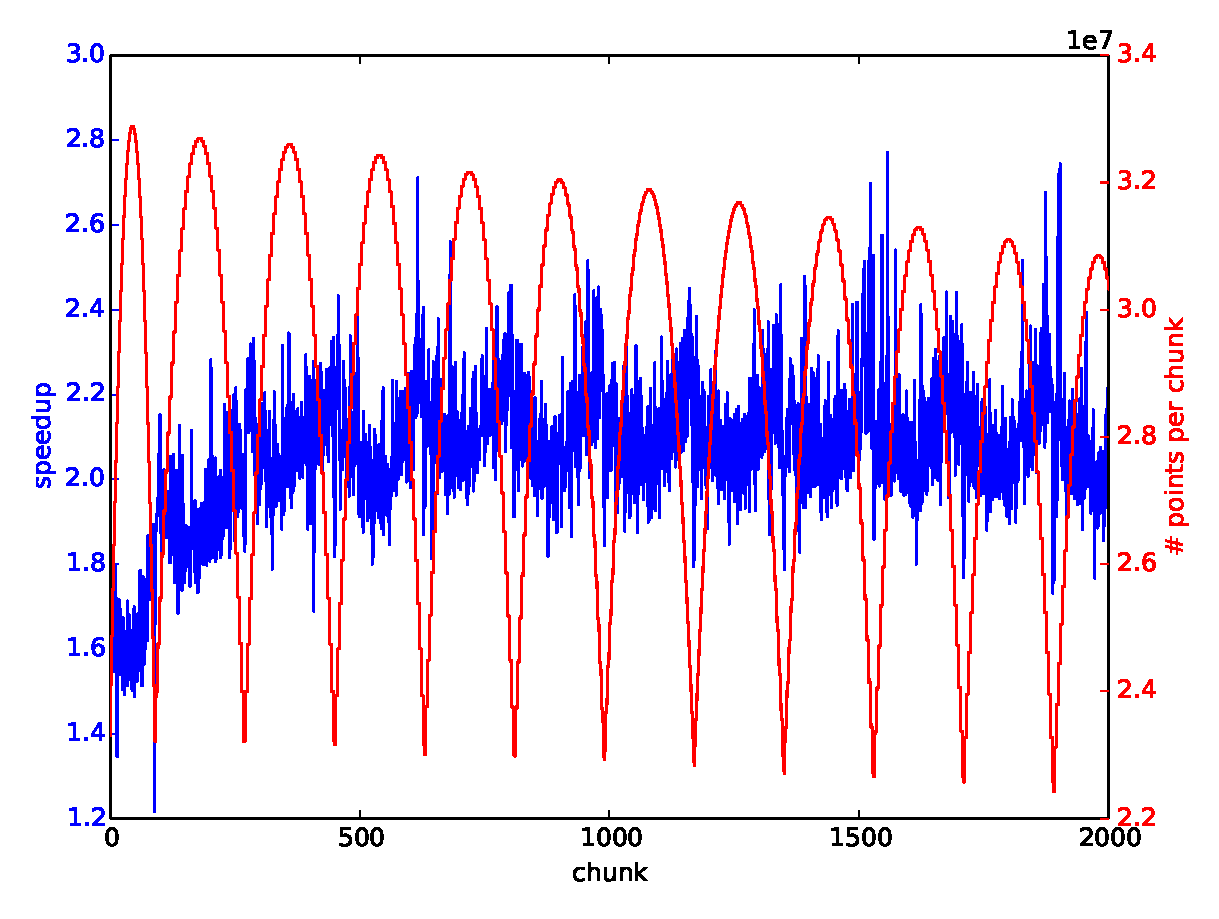
\includegraphics[width = 0.52\textwidth]{../speedup_2_iterations.pdf}\label{2its}}
      \caption{\textbf{left}: 6 iterations, \textbf{right}: 2 iterations}
  \end{figure}
  
  \begin{itemize}
    \item average speedup is similar
  \end{itemize}
\end{frame}

\begin{frame}
  \frametitle{}
  \begin{figure}
    \centering
      \subfloat[][]{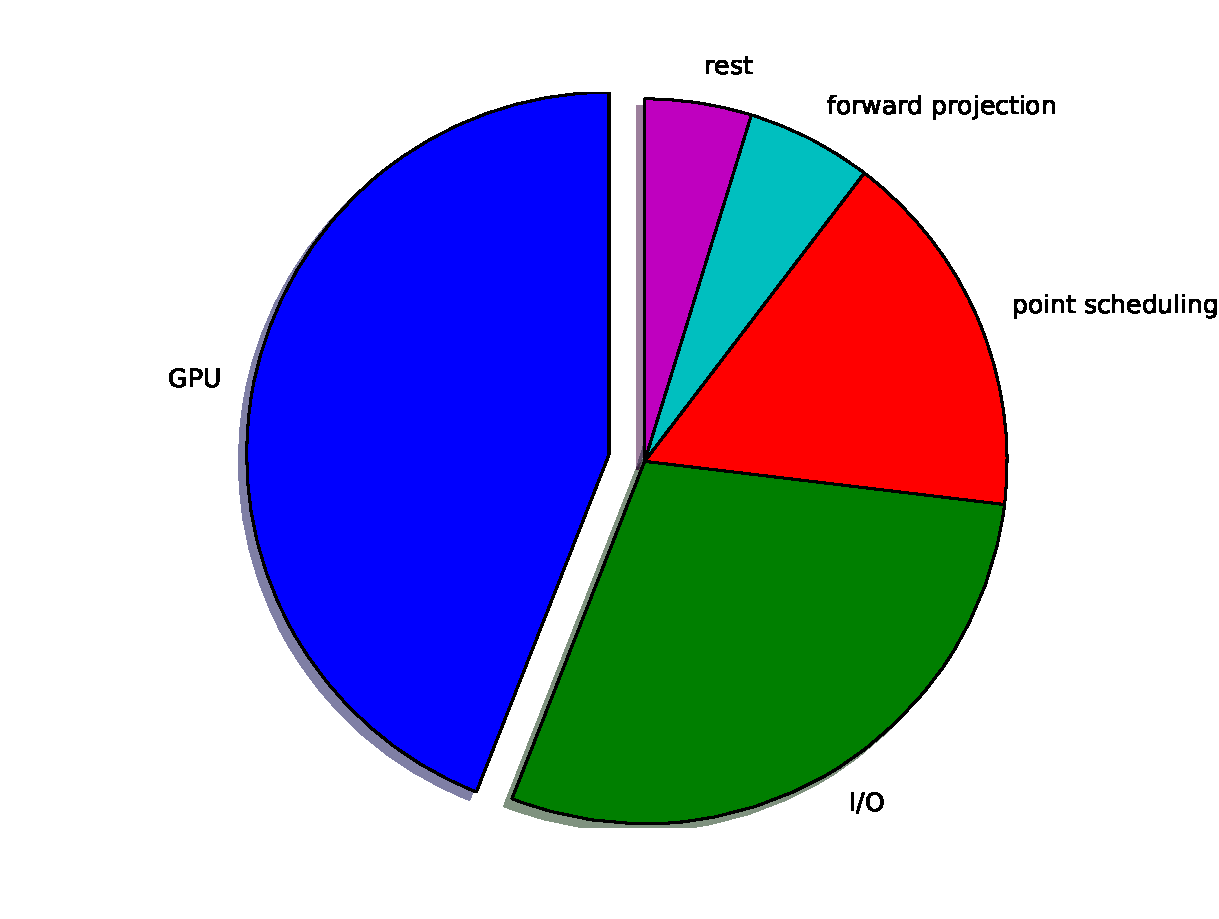
\includegraphics[width = 0.5\textwidth]{../forward_projection_time_distribution_6_iterations.pdf}\label{6its}}
      \subfloat[][]{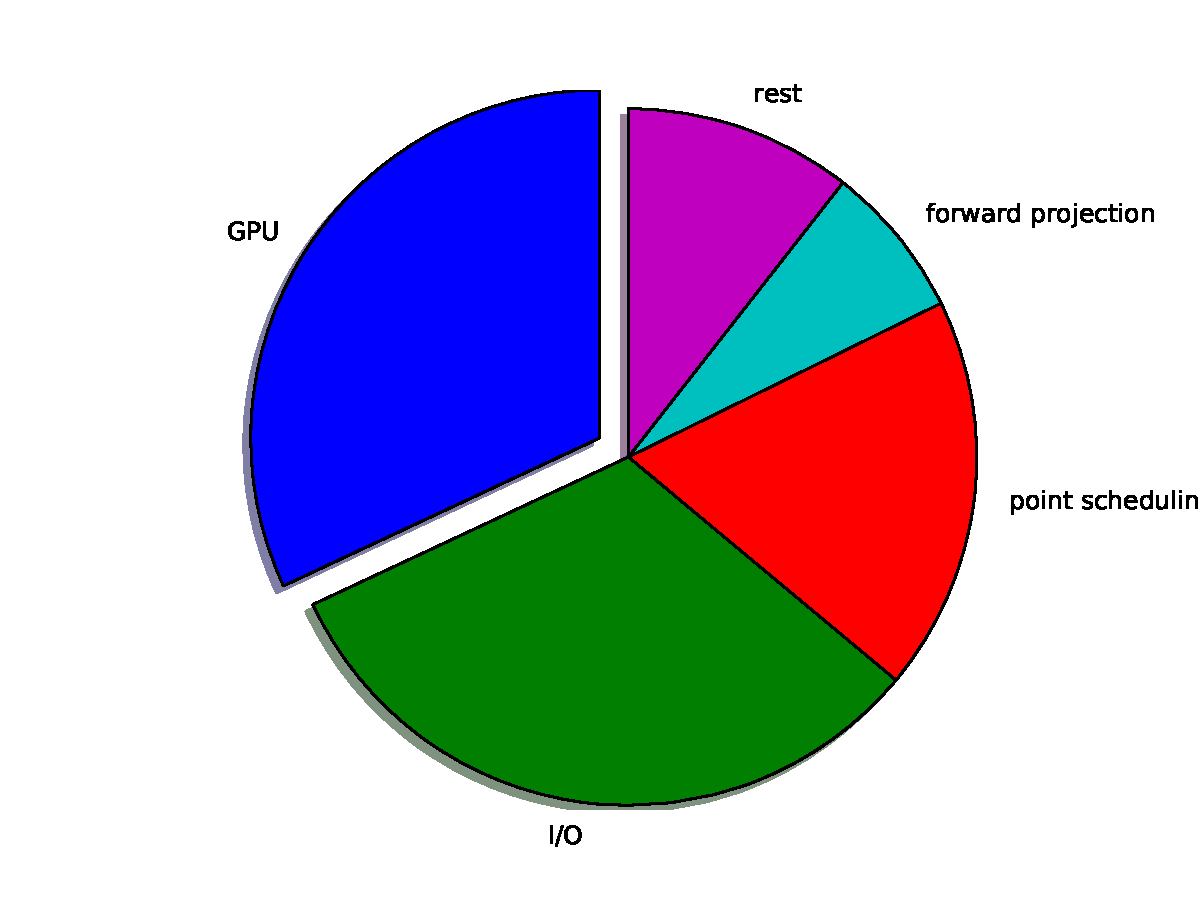
\includegraphics[width = 0.5\textwidth]{../forward_projection_time_distribution_2_iterations.pdf}\label{2its}}
      \caption{\textbf{left}: 6 iterations, \textbf{right}: 2 iterations}
  \end{figure}

  \begin{itemize}
    \item \textsl{I/O}: converting from \texttt{ProjMatrixElemsForOneBin} to \texttt{Tensor} and back
    \item \textsl{point scheduling}: choose points to sample the TOR / LOR
  \end{itemize}
\end{frame}

\begin{frame}
  \frametitle{Images}
  \begin{figure}
    \centering
    \subfloat[][]{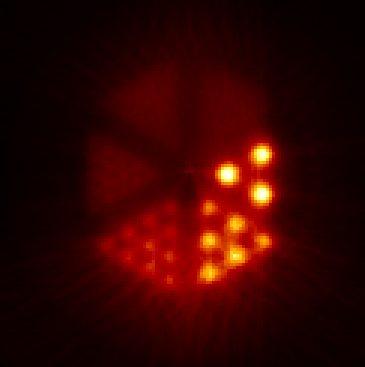
\includegraphics[height = 0.5\textwidth]{../2_iterations_20LORs.png}}
    \subfloat[][]{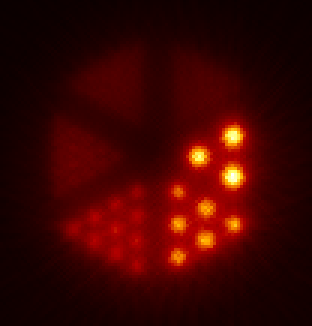
\includegraphics[height = 0.5\textwidth]{../Siddon_CPU.png}\label{2its}}
    \caption{\textbf{left}: 2 iterations, 20LORs per matrix element, \textbf{right}: original STIR}
  \end{figure}
  \begin{itemize}
    \item some artefacts: too few points
  \end{itemize}
\end{frame}

\begin{frame}
  \frametitle{How to proceed?}
  \begin{itemize}
    \item demonstrated a proof-of-concept of integrating Tensorflow into STIR
    \item whole toolchain is in place
      \begin{itemize}
        \item separation of graph generation (Python) and usage (C++) works very well
      \end{itemize}
    \item Speedup of $\sim$ 2 observed
  \end{itemize}

  Not too bad, but still some limitations:
  \begin{itemize}
    \item how to improve utilization of GPU (conversion between Tensors and STIR objects)?
    \item is there a better way to estimate the matrix elements?
    \item so far, use only a single thread (no \texttt{openMP} support)
      \begin{itemize}
        \item Tensorflow sessions tend to allocate all of the available GPU memory to avoid fragmentation...
      \end{itemize}
  \end{itemize}

\end{frame}

\begin{frame}
  \frametitle{Where to find the code?}
  \begin{itemize}
    \item STIR-TF: \url{https://github.com/philippwindischhofer/STIR/tree/stir-tf}
      \begin{itemize}
        \item in particular: \url{https://github.com/philippwindischhofer/STIR/blob/stir-tf/documentation/statistics/doc/main.pdf}
      \end{itemize}
    \item ray tracing scripts: \url{https://gitlab.phys.ethz.ch/luster/tf-raytracing} (ask Werner for access rights)
  \end{itemize}

  \begin{center}
    \textcolor{blue}{Any comments and contributions are welcome!}
  \end{center}

\end{frame}

\end{document}
